\documentclass{article}
\usepackage{fontspec}
\usepackage{xcolor}

\usepackage{amsthm}
\usepackage{amsmath}
\usepackage{amssymb}
\usepackage{unicode-math}
\usepackage[makeroom]{cancel}

\usepackage[normalem]{ulem}

\setmainfont{Times New Roman}
\setmathfont{Latin Modern Math}

\setlength\parindent{0em}
\setlength\parskip{0.618em}
\usepackage[a4paper,lmargin=1in,rmargin=1in,tmargin=1in,bmargin=1in]{geometry}

\usepackage{enumitem}

\renewcommand\qedsymbol{$\blacksquare$}

\usepackage{graphicx}

\begin{document}

\begin{center}
  \textbf{MATH} 148---\textbf{HOMEWORK} 5

  \color{red}R\color{teal}icardo
  \color{red}J\color{cyan}.
  \color{red}A\color{teal}cu$\color{red}{\widetilde{\color{teal}\text{n}}}$\color{teal}a\color{black}

  \color{teal}(\color{red}862079740\color{teal})\color{black}
\end{center}\vspace{1.618em}



\paragraph{1}  Consider a planar nonlinear system

\begin{cases}
x^\prime = y(y − 2)\\
y^\prime = x
\end{cases}

(1) For each equilibrium point, discuss if one can apply the Linearization Theorem to determine the local dynamics near it. If yes, sketch such local phase
portraits. If not, explain why it cannot be applied.

(2) Determine if the system is a Hamiltonian system. If yes, find its
Hamiltonian function.

(3) If it’s a Hamiltonian system, sketch the phase portraits via plotting the
level curves of the Hamiltonian function.

\textit{Hint: Compare this problem with example 2 of Chapter 4 that we did in class. You
  may need to switch the roles of x and y here.}

\uwave{Slu\enskip.}
\vspace{0.618 em}

(1)---

$(*)
\begin{cases}
0 = y(y − 2) = y^2 -2y\\
0 = x
\end{cases}$
$\implies (y=0$ or $y =2)$ and $x=0$

So, $\begin{pmatrix} 0\\ 0\end{pmatrix}$  and $\begin{pmatrix} 0\\
  2\end{pmatrix}$ are the equilibria of $(*)$.

Let $F(x, y) = \begin{pmatrix} y^2-2y\\
  x\end{pmatrix}$

$\implies DF(x,y) = \begin{pmatrix} 0 &
  2y -2 \\1 & 0\end{pmatrix}$

For $\begin{pmatrix} 0\\ 0\end{pmatrix}$:
$DF(0,0) = \begin{pmatrix} 0 &
  0 \\1 & 0\end{pmatrix}$ $\implies $Tr$(DF(0,0)) = 0$ and $|DF(0,0)|
= 0$.

So, $\begin{pmatrix} 0\\ 0\end{pmatrix}$ is a center. We cannot apply
the Linearization Theorem.

For $\begin{pmatrix} 0\\ 2\end{pmatrix}$:
$DF(0,2) = \begin{pmatrix} 0 &
  2 \\1 & 0\end{pmatrix}$ $\implies $Tr$(DF(0,0)) = 0$ and $|DF(0,0)|
= -2$.

So, $\begin{pmatrix} 0\\ 2\end{pmatrix}$ is a saddle. So we can apply
the Linearization Theorem.

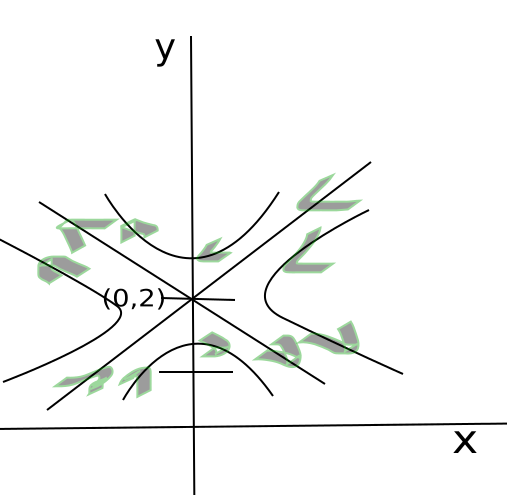
\includegraphics[width=0.25\textwidth]{saddle}
\newpage
(2)---

It is!

$H(x,y)= -\int y^2-2y\enskip dy +\int x\enskip dx = -\frac{y^3}{3} +y^2
+\frac{x^2}{2}$

Since, $x^\prime = -\frac{\partial H}{\partial y} = \frac{3y^2}{3} -2y
+0 = y(y-2)$ and $y^\prime = \frac{\partial H}{\partial x} = \frac{2x}{2} = x$

(3)---

$H^{-1}(C)= \{ x,y \in \mathbb{R}|\enskip -\frac{y^3}{3} +y^2
+\frac{x^2}{2} = C\}$

The constant can absorb the fractions. Equivalently:

$H^{-1}(C)= \{ x,y \in \mathbb{R}|\enskip -2y^3 +6y^2
+3x^2 = C\}$ $(**)$

We can express $x$ as a function of $y$:

$H^{-1}(C)= \{y \in \mathbb{R}|\enskip
f(y) = \pm\sqrt{\frac{C +2y^3 -6y^2}{3}}}\}$

So now we need to graph for different values of $C$, but reflect with
respect to the $x$ axis. I did that in my notebook, but I have a
computer so... I used expression $(**)$ in desmos.com to generate the
following phase-portrait.

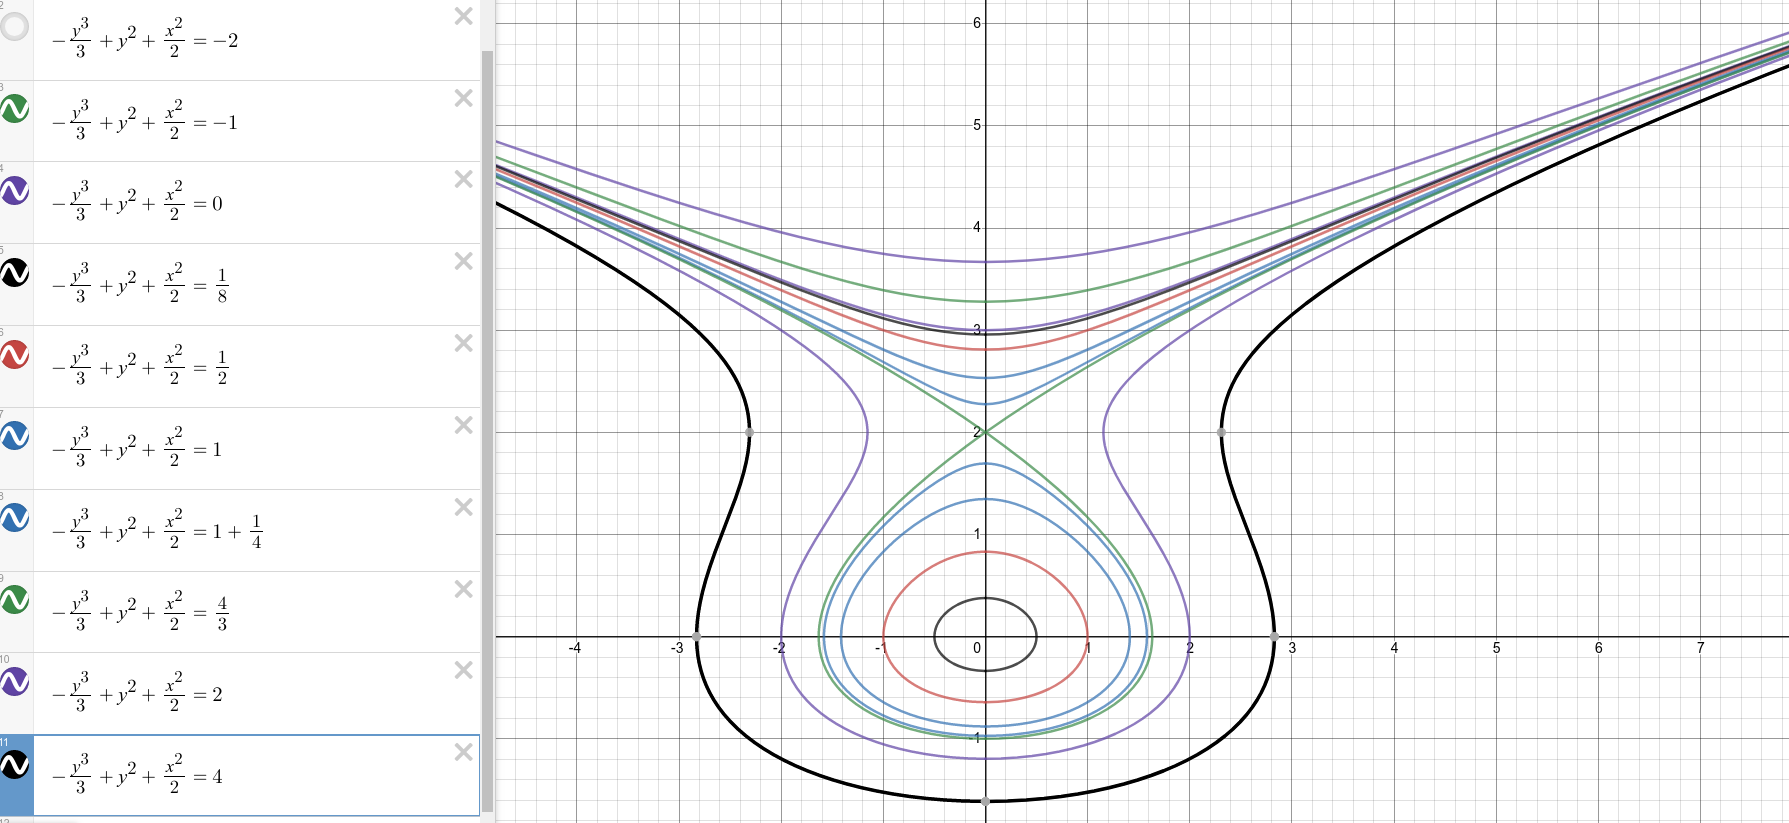
\includegraphics[width=\textwidth]{portrait}

Again in practice, we need to sketch the graph of $f(y)$ for different
values of $C$.

It's not defined when $\frac{C +2y^3 -6y^2}{3} = 0$ so
that's why we get disconnected chunks.




\newpage
\paragraph{2} Let $\vec{x_0}$ be an equilibrium point of a planar
dynamical system $Φ : \mathbb{R} ×
\mathbb{R}^2 → \mathbb{R}^2$
defined by a nice ODE system $\vec{x}^\prime = F(\vec{x})$. Recall that we say $\vec{x_0}$ is a sink if $\vec{0}$ is
a sink of the linearized system $\vec{u}^\prime = DF(\vec{x_0})\vec{u}$, where $\vec{u} = \vec{x} − \vec{x_0}$ and $DF(\vec{x_0})$ is
the derivative or Jacobian matrix of $F$ at $\vec{x_0}$. Similarly, we can define a source or
a saddle for a nonlinear system.

Let $Ψ$ be a dynamical system defined by $\vec{x}^\prime = G(\vec{x})$. Suppose $Φ$ is topologically
conjugate to $Ψ$ via homeomorphism $h$.

Suppose no eigenvalue of $DF(\vec{x_0})$ or $DG(
h(\vec{x_0}))$ has zero real part. In other
words, the linearized systems at both $\vec{x_0}$ and $h(\vec{x_0})$ are hyperbolic.
Show that $h(\vec{x_0})$ is a saddle if and only if $\vec{x_0}$ is a saddle. Show that the same
holds true if one replaces a saddle by a source or a sink. In other words, topological
conjugacy preserves the types of hyperbolic equilibria for nonlinear systems.

\textit{Hint: Previously, we did it for planar linear systems. Try to apply here the Linearization Theorem and the fact that topological conjugacy is an equivalence condition.
  Then you may reduce the nonlinear cases to linear cases.}

\uwave{Slu\enskip.}
\vspace{0.618 em}

Denote the dynamical systems corresponding to the Jacobians
DF$(\vec{x_0})$ and DG$(\vec{h(x_0)})$, respectively by $\Phi^l$ and
$\Psi^l$. Since, there exist a homomorphism $h$ for the conjugate
pairs $\Psi$ and $\Psi$, it follows that $h$ is a homomorphism of $\Phi^l$ and
$\Psi^l$ in a neighborhood around DF$(\vec{x_0})$ and DG$(\vec{h(x_0)})$ respectively.

($\impliedby$) Ass. $\vec{x_0}$ is a saddle of $\vec{x}^\prime = F(\vec{x})$

$W^s(\vec{0}) := \{\vec{x}\in \mathbb{R}^2| \vec{x} \neq
0$ and $\lim\limits_{t\rightarrow \infty}\Phi^l(t, \vec{x}) = \vec{0}\}$
and

$W^u(\vec{0}) := \{\vec{x}\in \mathbb{R}^2| \vec{x} \neq
0$ and $\lim\limits_{t\rightarrow -\infty}\Phi^l(t, \vec{x}) =
\vec{0}\}$


$\vec{0}$ is a saddle $\implies$ both  $W^s$ and $W^u$are not empty.

Since, $\Psi^l$ is conjugate to $\Phi^l$ via homomorphism $h$. It follows
that
$h\circ\Phi^l(t,\vec{x}) = \Psi^l(t,h(\vec{x}))$. It follows, that:

$W^s(\vec{h(0)}) := \{\vec{x}\in \mathbb{R}^2| \vec{x} \neq
0$ and $\lim\limits_{t\rightarrow \infty}h\circ\Phi^l(t, \vec{x})
= \Psi^l(t,h(\vec{x})) = h(\vec{0})\}$
and

$W^u(\vec{h(0)}) := \{\vec{x}\in \mathbb{R}^2| \vec{x} \neq
0$ and $\lim\limits_{t\rightarrow -\infty} h\circ\Phi^l(t, \vec{x}) =\Psi^l(t,h(\vec{x}))
= h(\vec{0})\}$

are both non-empty, as $h$ is continuous and bijective.

So, $h(\vec{x_0})$ a saddle of $\vec{x}^\prime = G(\vec{x})$

($\implies$) Ass. $h(\vec{x_0})$ is a saddle of $\vec{x}^\prime = G(\vec{x})$

Since, $\Psi^l$ is conjugate to $\Phi^l$ via homomorphism $h$. There
exists a continuous inverse $h^{-1}$ of $h$. It follows
that $\Psi^l$ is conjugate to $\Phi^l$ via $h^{-1}$. So, $h^{-1}\circ
\Psi^l(t,h(\vec{x})) = \Phi^l(t,h^{-1}\circ h(\vec{x})) = \Phi^l(t,\vec{x})$ .

Since $h(\vec{0})$ a saddle

$W^s(\vec{h(0)}) := \{\vec{x}\in \mathbb{R}^2| \vec{x} \neq
0$ and $\lim\limits_{t\rightarrow \infty} \Psi^l(t,h(\vec{x})) = h(\vec{0})\}$
and

$W^u(\vec{h(0)}) := \{\vec{x}\in \mathbb{R}^2| \vec{x} \neq
0$ and $\lim\limits_{t\rightarrow -\infty}  \Psi^l(t,h(\vec{x}))
= h(\vec{0})\}$


are both non-empty.

Via the conjugacy $h^{-1}$ we obtain the following sets:

$W^s(\vec{0}) = W^s(h^{-1}\circ h(\vec{0})) = \{\vec{x}\in \mathbb{R}^2| \vec{x} \neq
0$ and $\lim\limits_{t\rightarrow \infty} h^{-1}\circ
\Psi^l(t,h(\vec{x})) = \Phi^l(t, \vec{x}) = \vec{0}\}$
and

$W^u(\vec{0}) = W^s(h^{-1}\circ h(\vec{0})) = \{\vec{x}\in \mathbb{R}^2| \vec{x} \neq
0$ and $\lim\limits_{t\rightarrow -\infty} h^{-1}\circ
\Psi^l(t,h(\vec{x})) = \Phi^l(t, \vec{x}) = \vec{0}\}$

Since $h^{-1}$ is a continuous bijection, these sets are not
empty.

So, $\vec{x_0}$ is a saddle of $\vec{x}^\prime = F(\vec{x})$

Similarly, it is clear that the homomorphism preserves the type of the
systems, because the type changes depending only on whether the
initial sets $W^s$ and $W^u$ are initially empty. The argument breaks
only in the case when both $W^s$ and $W^u$ are empty, as the center
type doesn't give any information for the Linearization Theorem.
\vspace{0.618 em}
$\blacksquare$


\newpage
3. For a planar linear system $\vec{x}^\prime = A\vec{x}$ with $A = \begin{bmatrix}
a& b\\
c& d \end{bmatrix}$
, determine for what choices
of $a, b, c, d ∈ \mathbb{R}$, it’s a Hamiltonian system. Assume in addition that $|A| \neq 0$. Then
without using the Liouville’s Theorem, explain why $\vec{0}$ cannot be a sink or source
for such choices of $a, b, c, d$. Or equivalently, why $\vec{0}$ can only be a center or a saddle
point in such system.

\uwave{Slu\enskip.}
\vspace{0.618 em}


$(***)
\begin{cases}
x^\prime = ax+by\\
y^\prime = cx+dy
\end{cases}$

$
(***)$ is Hamiltonian $\iff \frac{\partial ax+by}{\partial x} =
-\frac{\partial cx+dy}{\partial y}\quad [1]
$


$\implies a = -d$

So, $a, b,$ and $c$ are free variables. However, $d = -a$ as $[1]$ is
an iff statement.

$\implies A = \begin{pmatrix}a& b\\ c& -a\end{pmatrix} \implies$ Tr$(A)=0$


$|A| \neq 0 \implies |A| < 0$ or $ 0 < |A|$

Case I: $|A| < 0$ and Tr$(A) = 0$
$\implies \vec{0}$ is a saddle of $(***)$

Case I: $0 < |A|$ and Tr$(A) = 0$
$\implies \vec{0}$ is a center of $(***)$

\vspace{0.618 em}
$\blacksquare$

\end{document}
%%% Local Variables:
%%% mode: latex
%%% TeX-master: t
%%% End:
